\section{RASD}

	\begin{frame}[plain]
		\vfill
		\centering
		\begin{beamercolorbox}[sep=8pt,center,shadow=true,rounded=true]{title}
			\textbf{\usebeamerfont{title}\insertsectionhead}\par%
			\color{polimiblue}\noindent\rule{10cm}{1pt} \\
		\end{beamercolorbox}
		\vfill
	\end{frame}

	\subsection{Goals}
		\begin{frame}{Goals}
			\vspace{-17pt}
			\begin{enumerate}[label=\textbf{G\arabic*}]\small
				\item \label{goal:notification} Users should be able to notify authorities when traffic violations occur, in particular parking violations.
				\item \label{goal:mining} Users and authorities should be able to mine the information stored by SafeStreets, with different levels of visibility.
				\begin{enumerate}[label=\textbf{G2\Alph*}]
					\item \label{goal:miningA} Users and authorities should be able to know where the highest number of violations occur.
					\item \label{goal:miningB} Users and authorities should be able to know what types of vehicle make the most violations.
					\item \label{goal:miningC} Authorities should be able to consult every violation report sent by users.
				\end{enumerate}
				\item \label{goal:safety} Users and authorities should be able to know which streets are safe and which ones are not.
				\item \label{goal:intervention} Users and authorities should be able to know the possible interventions that could be done in a city.
			\end{enumerate}
		\end{frame}

	\subsection{Boundaries of the system}
		\begin{frame}{System Interfaces}
			\vspace{-10pt}
			We want now to define the boundaries of our system first with the external interfaces it has to interact with, second with the \emph{World And Machine} that helps to highlight the phenomena.
			
			\begin{figure}[h!]
				\centering
				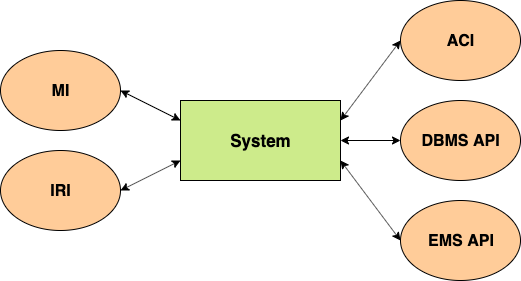
\includegraphics[scale=0.48]{rasd/externalInterfaces.png}
			\end{figure}
		\end{frame}
		
		\begin{frame}{The World and the Machine}
			\vspace{-24pt}
			\begin{figure}[hbtp]
				\centering
				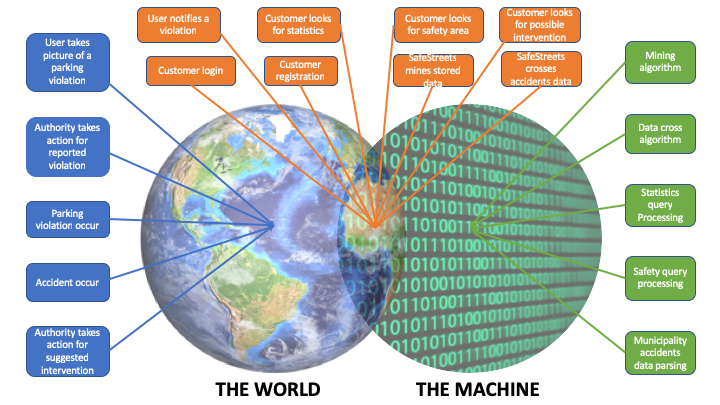
\includegraphics[scale=0.33]{rasd/WorldAndMachine}
			\end{figure}
		\end{frame}
	
	\subsection{Meaningful Use-Cases}
		\begin{frame}{Use Case and Authority Registration}
			\hspace*{-0.7cm}
			\begin{minipage}{0.4\textwidth}
				\centering
				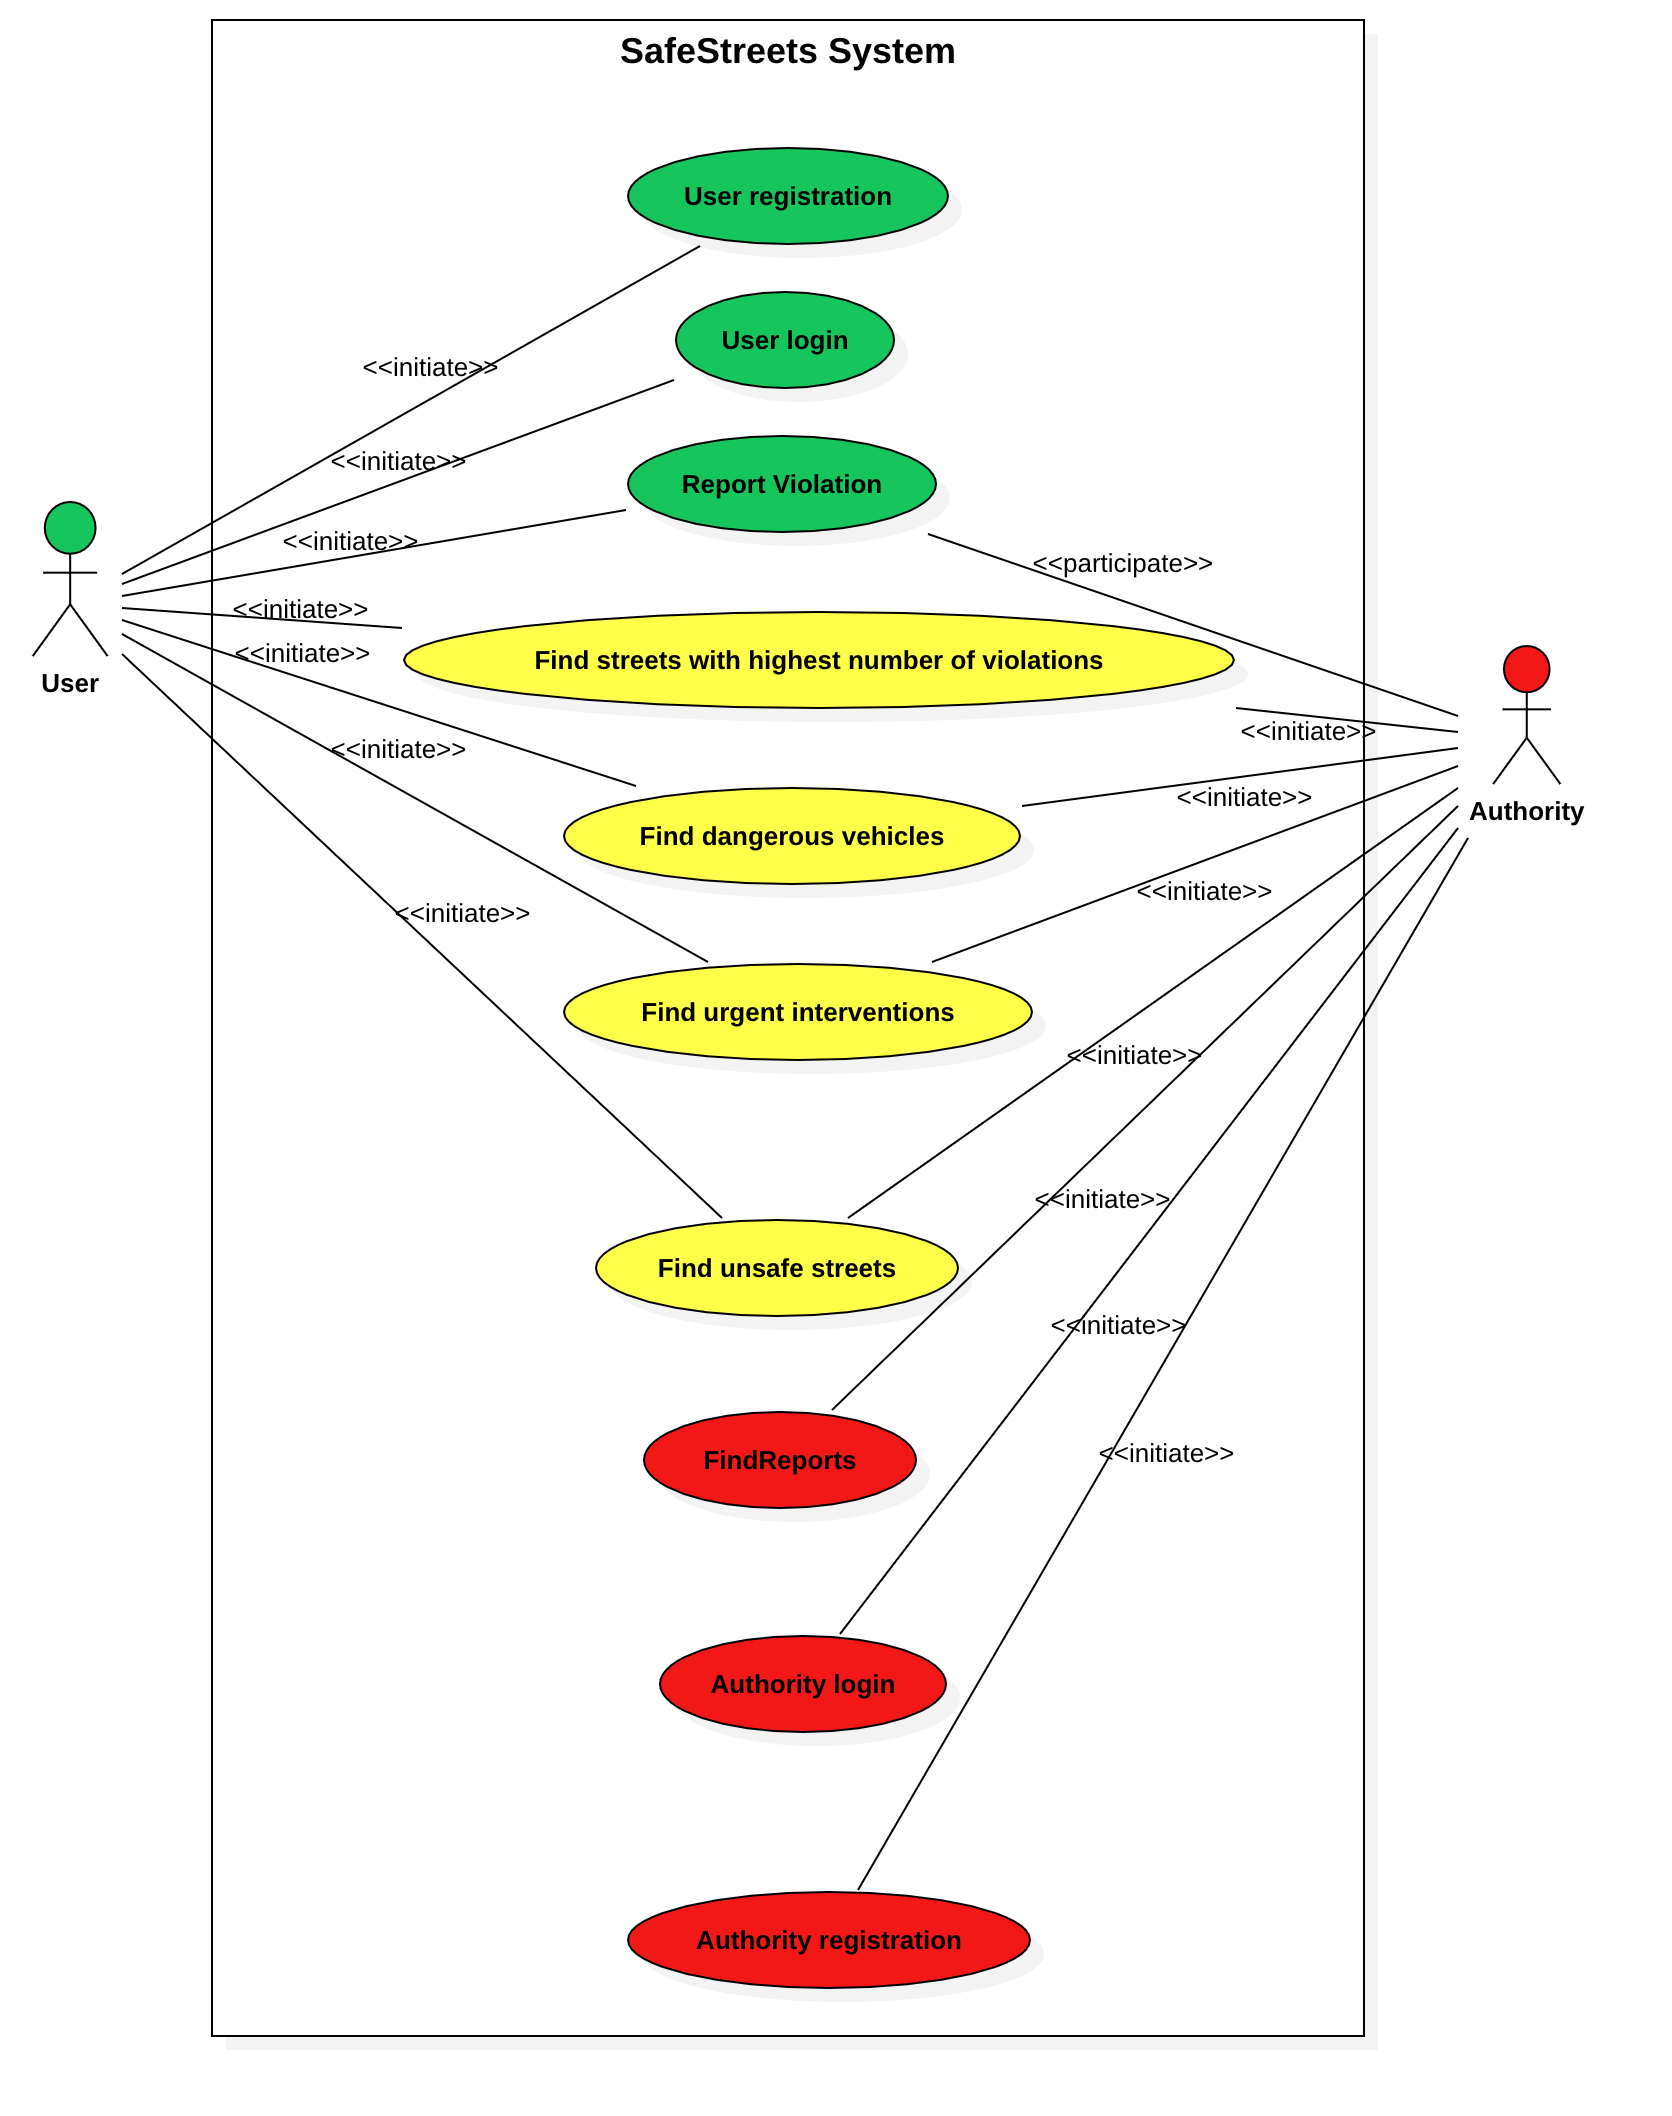
\includegraphics[scale=0.1]{rasd/useCaseDiagramModel}
			\end{minipage}\hspace{1.9cm}
			~
			\begin{minipage}{0.4\textwidth}
				\centering
				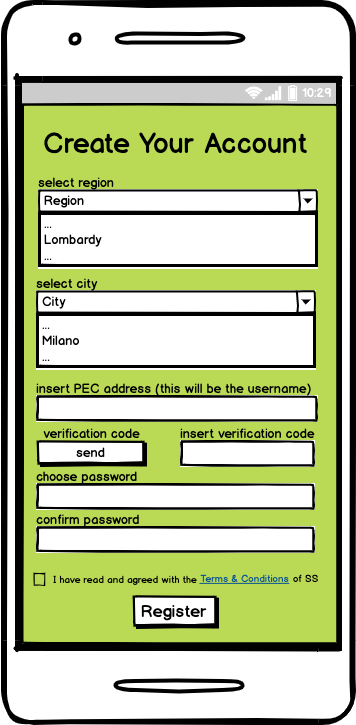
\includegraphics[scale=0.104]{rasd/authorityRegistration}
			\end{minipage}
		\end{frame}
	
		\begin{frame}{Report Violation and Unsafe Streets}
			\hspace*{-0.4cm}
			\begin{minipage}{0.4\textwidth}
				\centering
				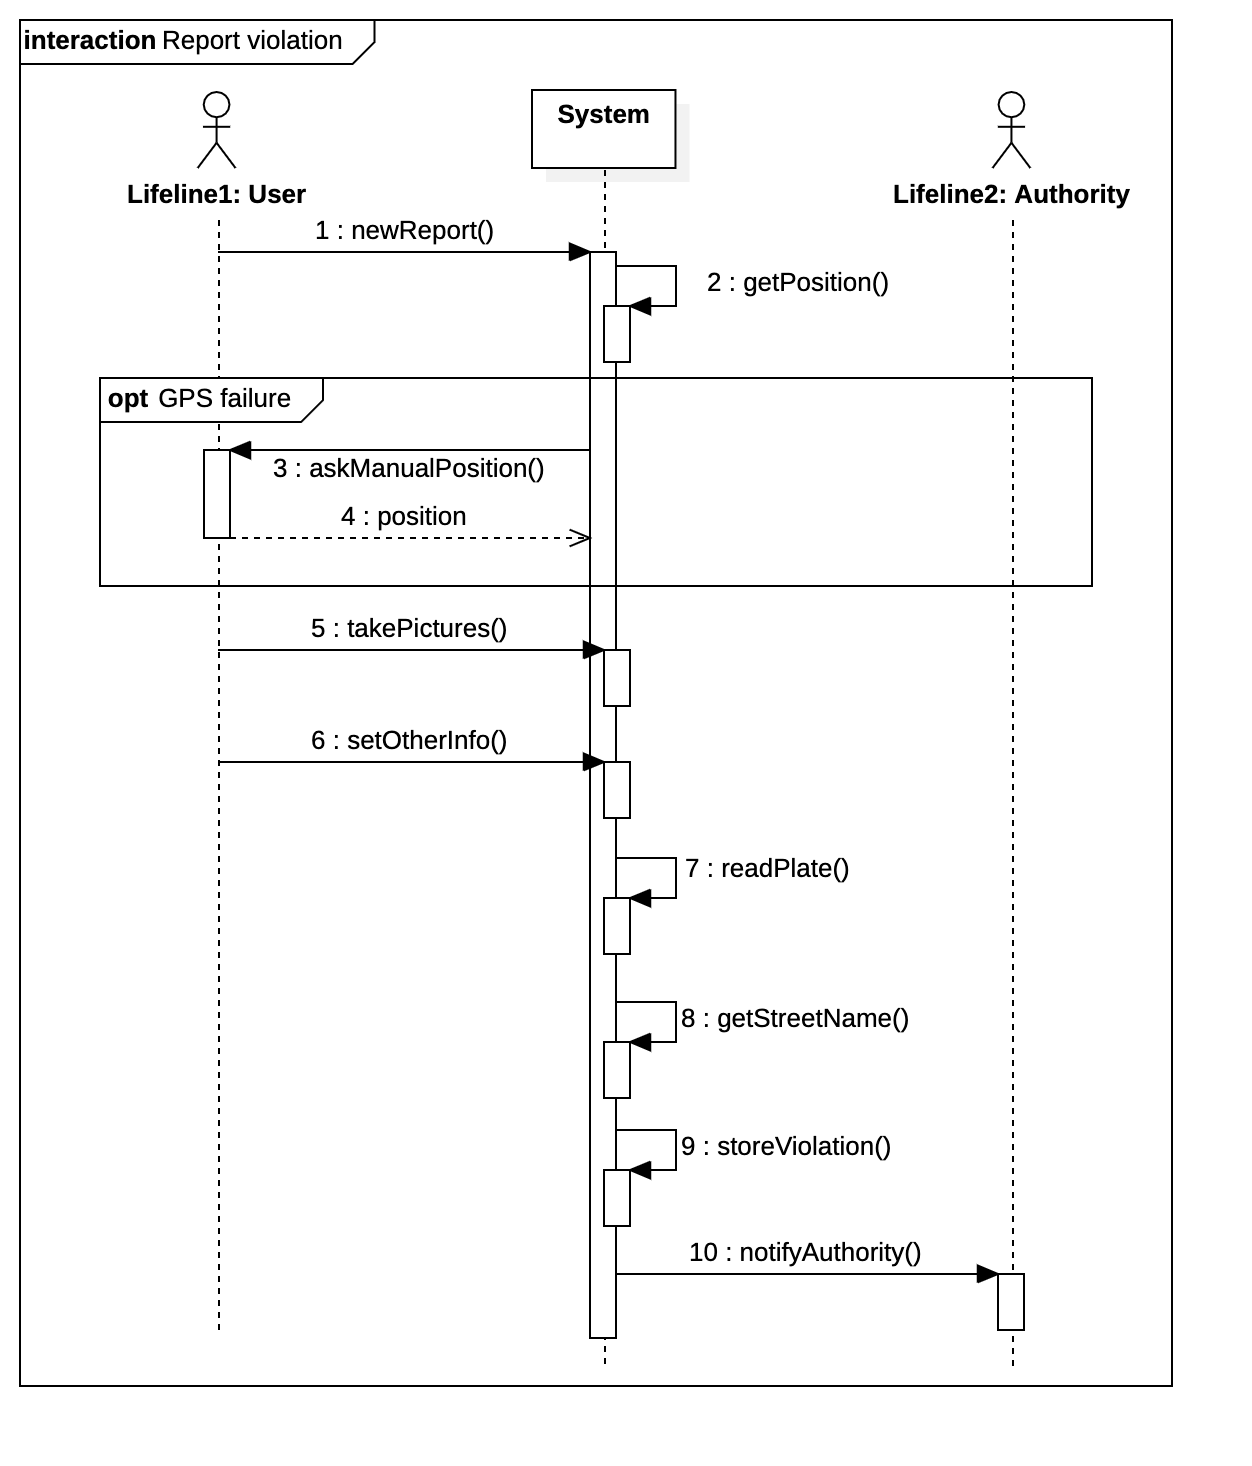
\includegraphics[scale=0.13]{rasd/reportViolation}
			\end{minipage}\hspace{1.2cm}
			~
			\begin{minipage}{0.4\textwidth}
				\centering
				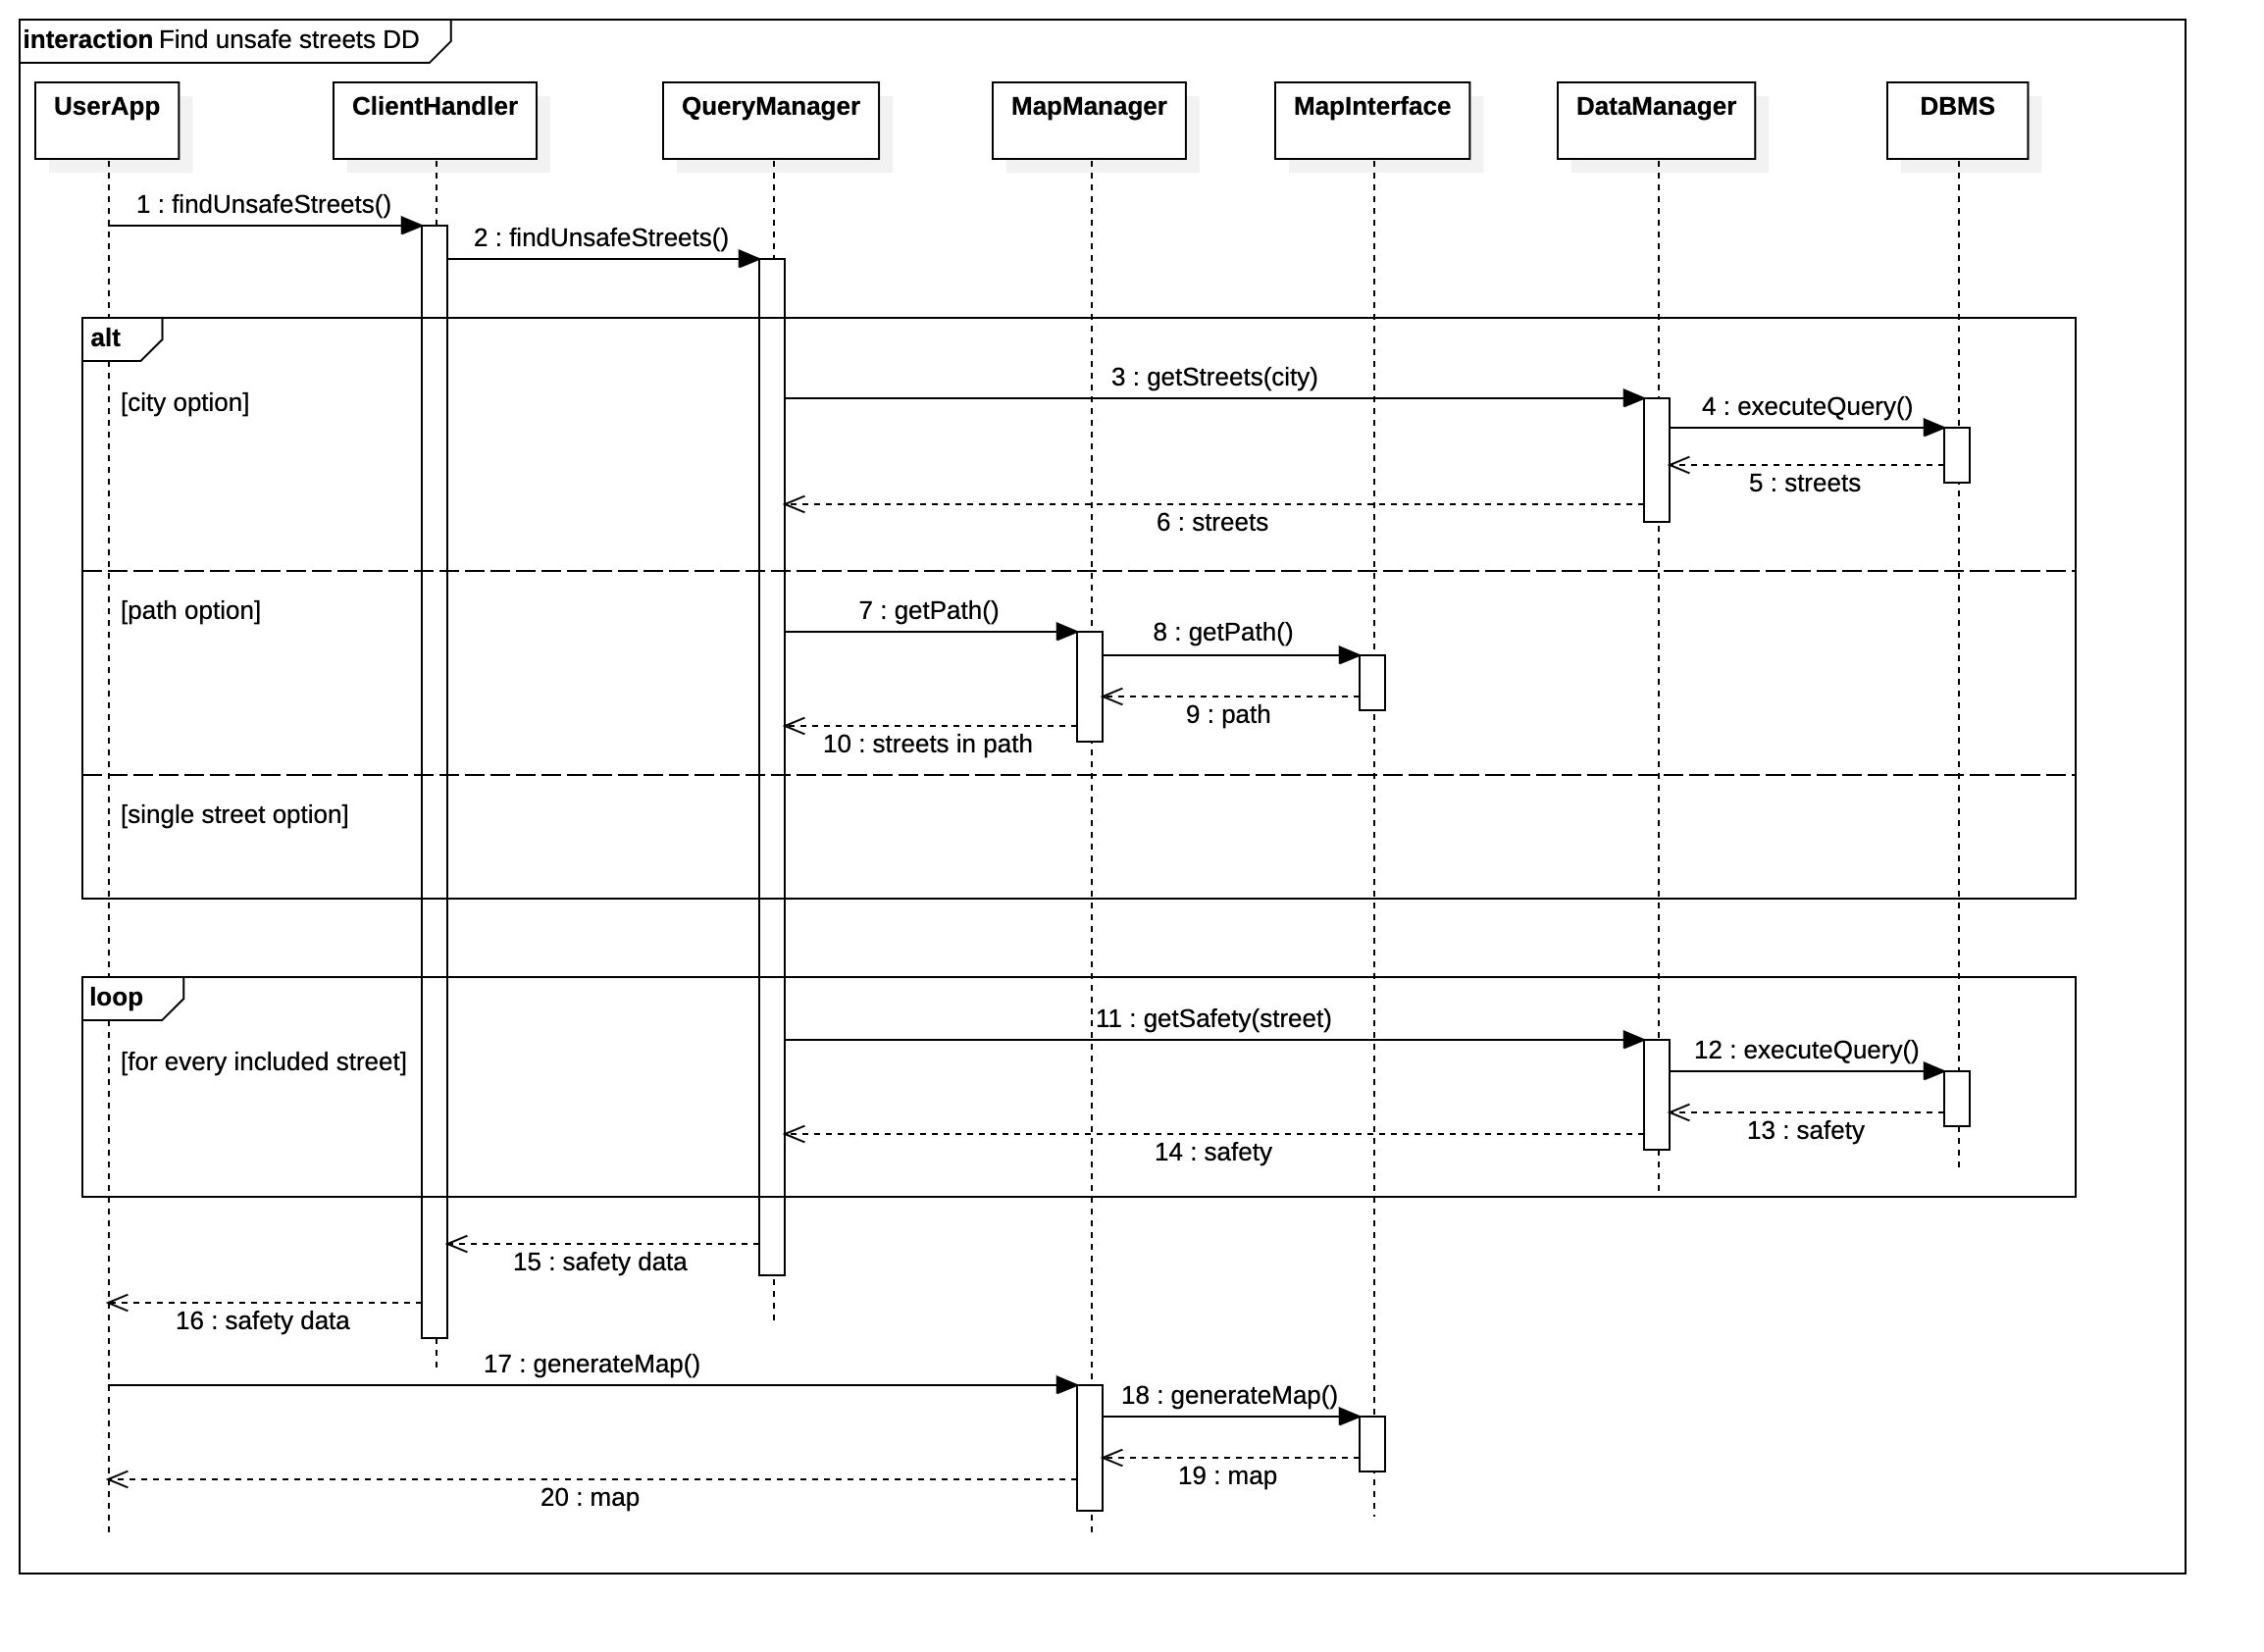
\includegraphics[scale=0.123]{rasd/unsafeStreets}
			\end{minipage}
		\end{frame}
	
	\subsection{Relevant Requirements}
		\begin{frame}{Relevant Requirements}
			\begin{itemize}
				\item <1-> \textbf{R8} The system must allow users to take pictures of the violation they want to report
				
				\item <2-> \textbf{R17} The system must be able to show authorities all the violation reports sent by users
				
				\item <3-> \textbf{R18} The system must be able to mine the stored violation reports
				
				\item <4-> \textbf{R31} The system must be able to determine whether a street is safe or not
				
				\item <5-> \textbf{R35} The system must be able to determine the most urgent interventions in a street.
			\end{itemize}
		\end{frame}
	
	\subsection{Relevant Assumptions}
		\begin{frame}{Relevant Assumptions}
			\begin{itemize}
				\item <1-> \textbf{DA2} Users always insert correct data while reporting violations to SafeStreets
				
				\item <2-> \textbf{DA7} The GPS module of the devices on which SafeStreets runs always works correctly and has an accuracy of 2 meters
				
				\item <3-> \textbf{DA8} The camera module of the devices on which SafeStreets runs always works correctly
				
				\item <4-> \textbf{DA10} The system is assumed to work in Italy
				
				\item <5-> \textbf{DA13} No one physically and maliciously replaces license plates
				
				\item <6-> \textbf{DA17} Accidents data provided by municipalities are always correct
			\end{itemize}
		\end{frame}

	\subsection{Alloy Model}
		\begin{frame}{First World}

			\begin{figure}[hbtp]
				\centering
				\hspace*{-0.9cm}
				\vspace*{2.5cm}
				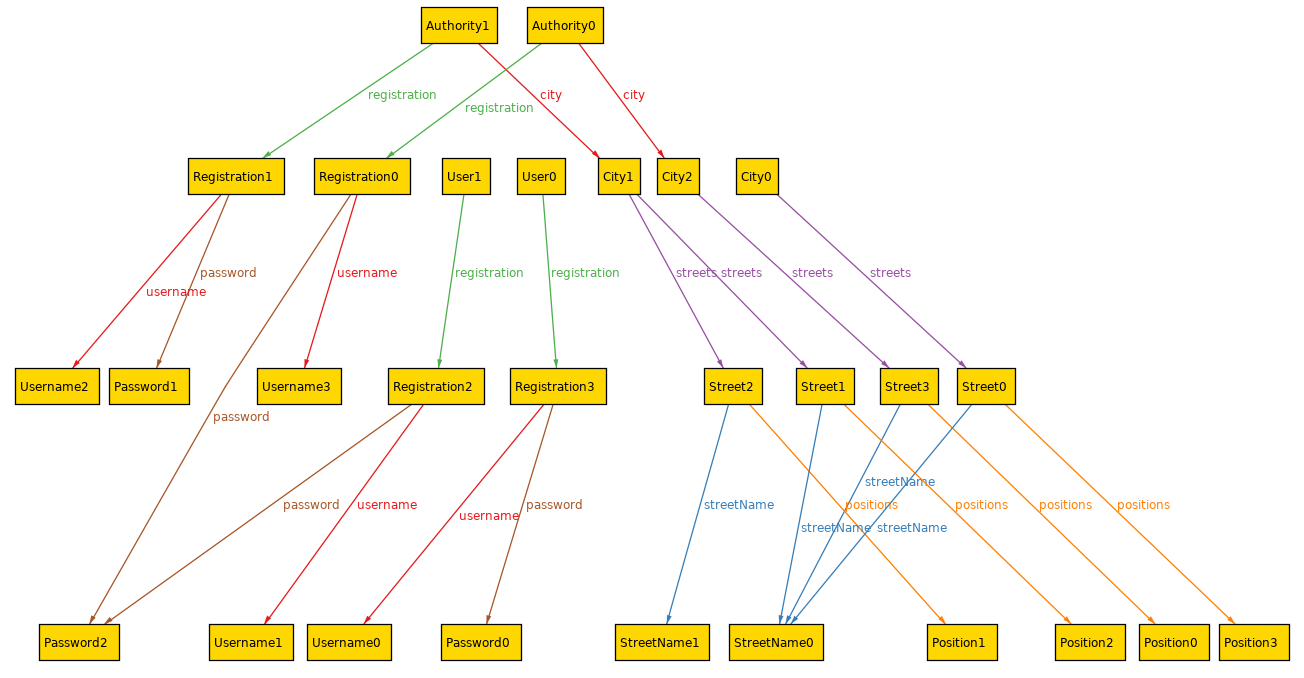
\includegraphics[scale=0.27]{rasd/world1}
			\end{figure}
		\end{frame}
	
		\begin{frame}{Second World}
			\vspace*{-1.5cm}
			\begin{figure}
				\centering
				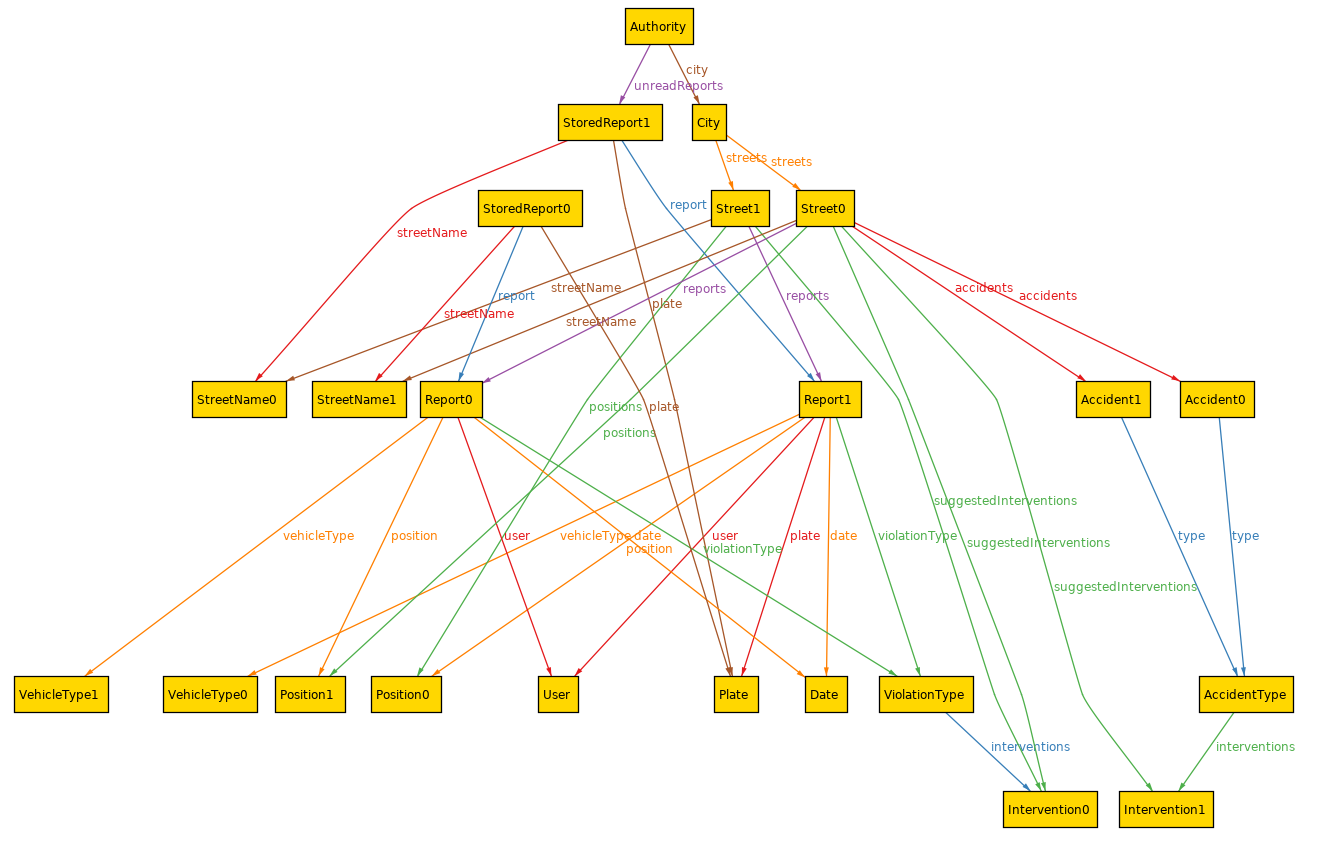
\includegraphics[scale=0.25]{rasd/world2}
			\end{figure}
		\end{frame}
	
		\begin{frame}{Facts}
			\begin{minipage}{0.4\textwidth}
				\centering
				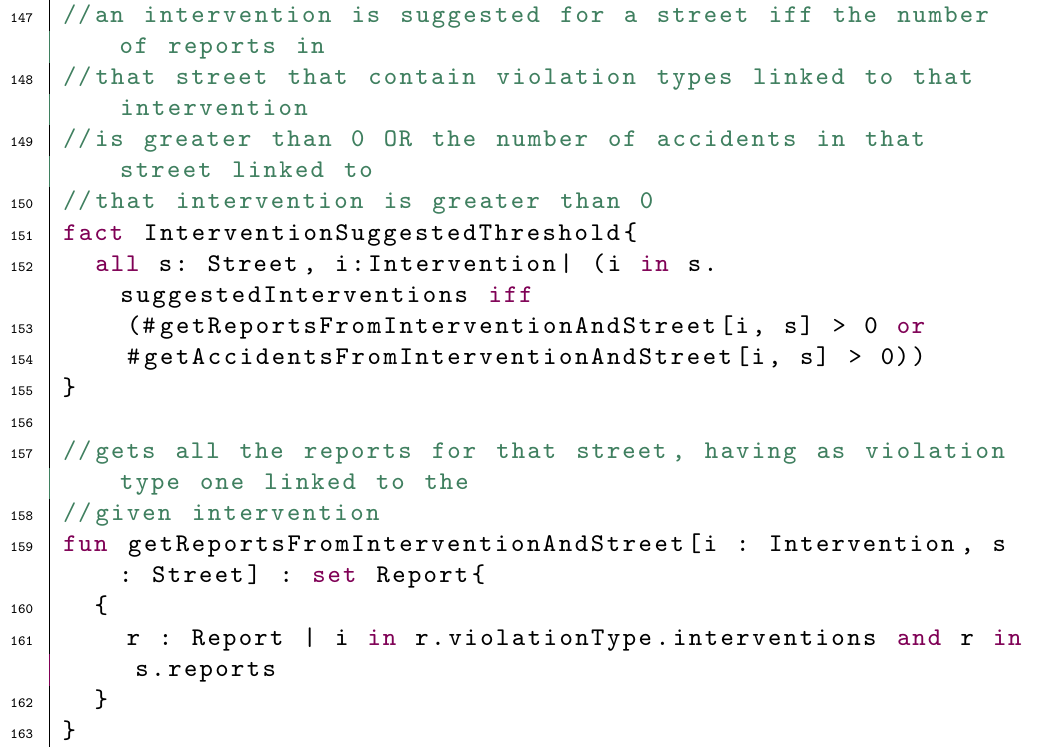
\includegraphics[scale=0.23]{rasd/interventionSuggestedThreshold}
			\end{minipage}\hspace{0.5cm}
		\end{frame}

		\begin{frame}{Facts}
			\begin{minipage}{0.4\textwidth}
				\centering
				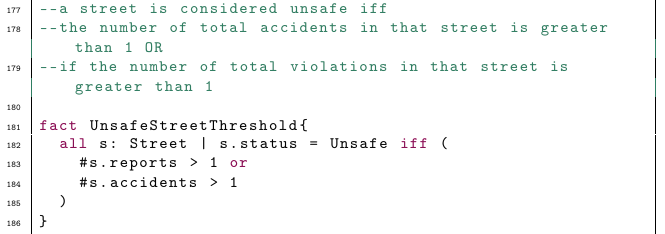
\includegraphics[scale=0.45]{rasd/unsafeStreetThreshold}
			\end{minipage}\hspace{0.5cm}
		\end{frame}
	
		\begin{frame}{Third World}
			\begin{minipage}{0.4\textwidth}
				\centering
				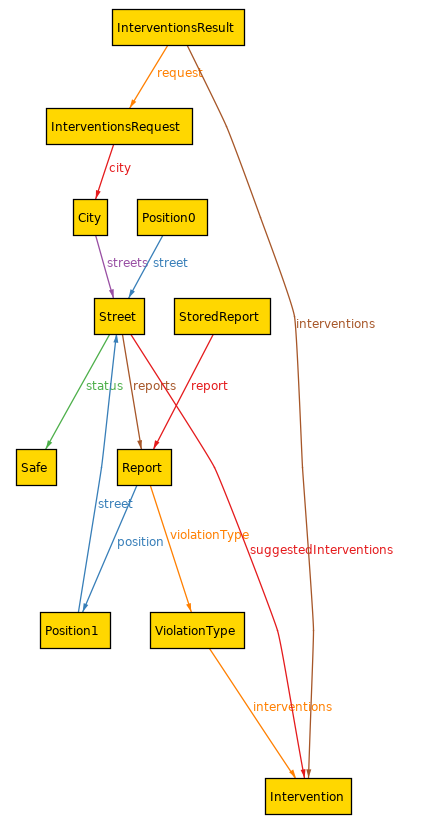
\includegraphics[scale=0.23]{rasd/world3}
			\end{minipage}\hspace{0.5cm}
			~
			\begin{minipage}{0.4\textwidth}
				\centering
				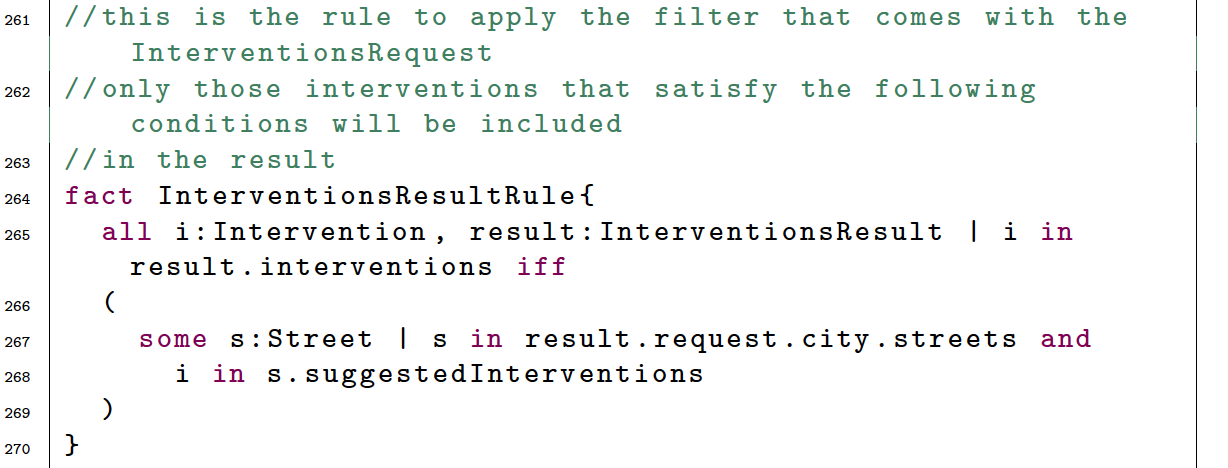
\includegraphics[scale=0.3]{rasd/interventionsResultRule}
			\end{minipage}
		\end{frame}
	
		\begin{frame}{Facts}
			\begin{minipage}{0.4\textwidth}
				\centering
				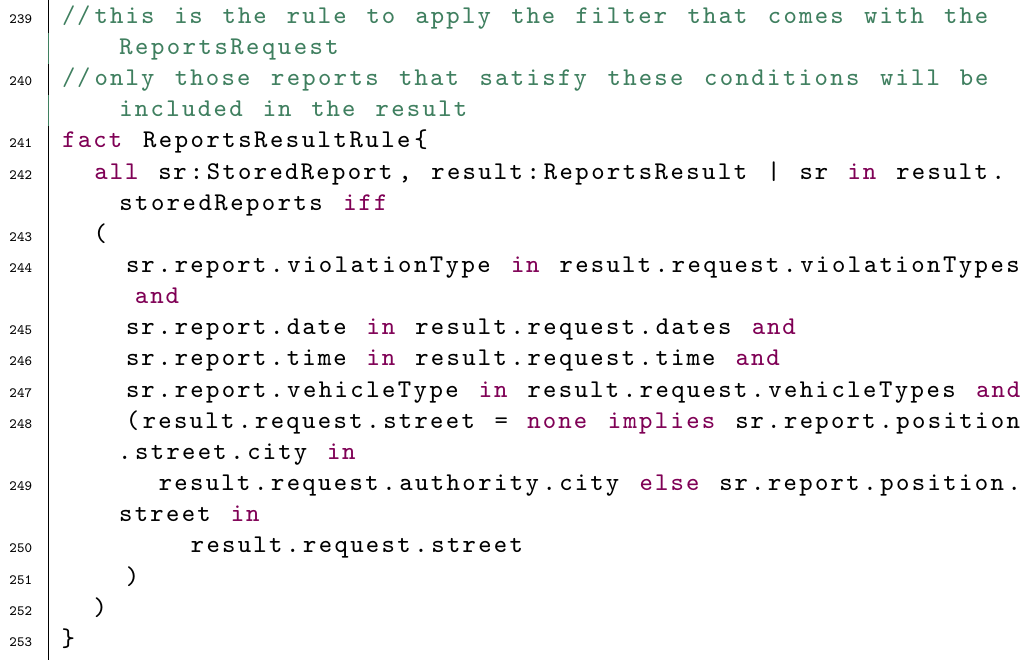
\includegraphics[scale=0.29]{rasd/reportsResultRule}
			\end{minipage}\hspace{0.5cm}
		\end{frame}